\documentclass[11pt,tikz]{standalone}

\begin{document}
\def\width{120}
\def\height{140}
\def\margin{10}
\def\tbheight{90}
\def\hbheight{20}

\tikzset{x=1pt, y=-1pt, layout/.style={line width=5pt, lightgray, line cap=round}, nonfocus/.style={lightgray}}

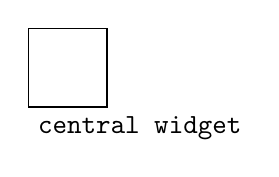
\begin{tikzpicture}
  \draw (0, 0) node[below right] {\texttt{central widget}} rectangle (\width, \height);
\end{tikzpicture}
\begin{tikzpicture}
  \draw (0, 0) node[below right] {\texttt{vbox}} rectangle (\width, \height);
  \foreach \i in {.75, 1.75, 2.75} {
      \draw[layout] (\margin, {\i * (\height - 2 * \margin) / 3 + \margin}) -- +(\width - 2 * \margin, 0);
    }
\end{tikzpicture}
\begin{tikzpicture}
  \draw[nonfocus] (0, 0) rectangle (\width, \height);
  \draw (\margin, \margin) node[below right] {\texttt{textbox}} rectangle +(\width - 2 * \margin, \tbheight);
  \begin{scope}[yshift=-(\tbheight + 2 * \margin)]
    \foreach \i in {.5, 1.5, 2.5} {
        \draw[layout] ({\i * (\width - 2 * \margin) / 3 + \margin}, 5) -- +(0, \hbheight - 10);
      }
  \end{scope}
  \draw (\margin, \tbheight + 2 * \margin) node[below right,fill=white] {\texttt{hbox}} rectangle +(\width - 2 * \margin, \hbheight);
\end{tikzpicture}
\begin{tikzpicture}
  \draw[nonfocus] (0, 0) rectangle (\width, \height);
  \draw[nonfocus] (\margin, \margin) rectangle +(\width - 2 * \margin, \tbheight);
  \begin{scope}[yshift=-(\tbheight + 2 * \margin)]
    \node[draw] at (.3 * \width, .5 * \hbheight) {\texttt{button}};
    \node[draw] at (.7 * \width, .5 * \hbheight) {\texttt{button}};
  \end{scope}
  \draw[nonfocus] (\margin, \tbheight + 2 * \margin) rectangle +(\width - 2 * \margin, \hbheight);
\end{tikzpicture}
\end{document}